% !TEX root = Modi_RobustCode.tex

\chapter[S자 이야기]{S자 이야기(Letter S)}


\begin{flushright}
\small\sffamily 이 글은 도널드 크누스가 쓴 \emph{Digital Typography}(CSLI, 1999)에서 발췌하였다. 
\end{flushright}


\noindent 도널드 크누스(Donald E. Knuth) 교수가 쓴
    \href{http://www-cs-faculty.stanford.edu/~knuth/dt.html}{\emph{Digital Typography}}에
    재미있는 꼭지가 있습니다. ``S자 이야기(The Letter S)''인데요,
    프란체스코 토르니엘로(Francesco Torniello)라는 이탈리아의 한
    타이포그래퍼가 쓴 알파벳 도해법에서 S자 도해를 수학적으로 계산하여
    설명하고 있습니다. 재미있는 부분이라는 생각이 들어서 조금
    인용해봅니다. 원문 그대로 옮기지는 않았고요, 제가 중간중간에
    이해를 돕기 위해 추가한 부분이 있습니다만 따로 명기하지는
    않았습니다. 


\section{S자 이야기 중}
 
몇 년 전 최신 프린트 장비에 사용할 적당한 알파벳을 디자인해야하는
문제가 있었는데 문자 스물다섯 개는 비교적 다루기가 쉬웠다. 그렇지 않은
다른 하나는 바로 `S'자였다.
\medskip

(중략)
\bigskip
\begin{figure}
\centering{%
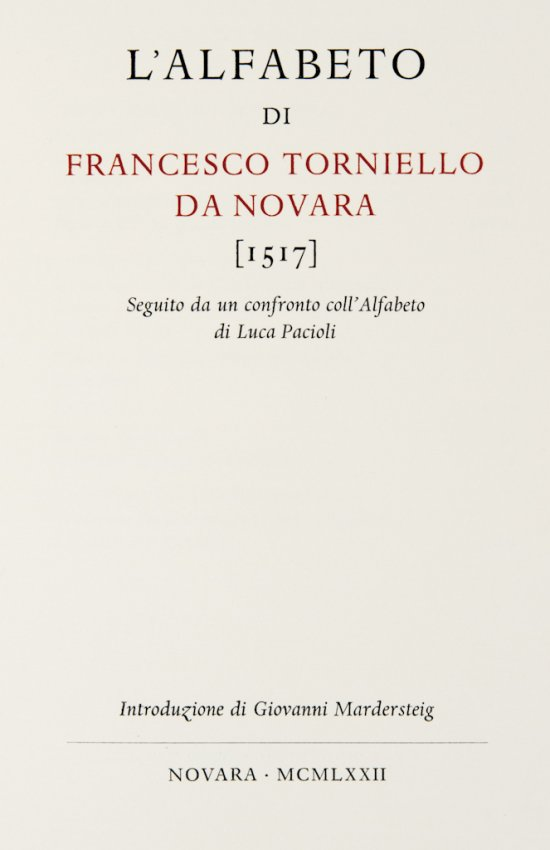
\includegraphics[width=.35\textwidth]{pictures/LAlfabeto}\qquad
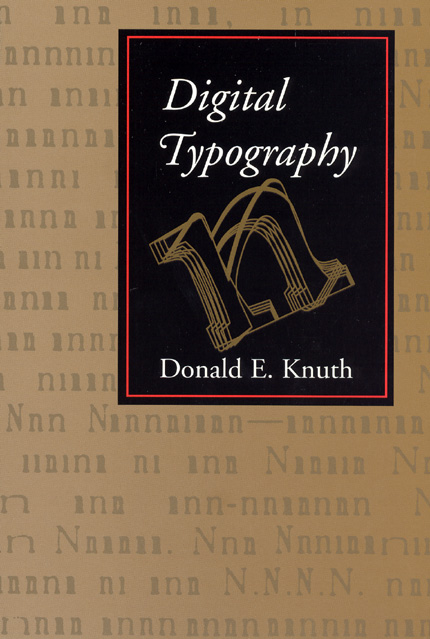
\includegraphics[width=.35\textwidth]{pictures/DigitalTypography}
\caption{프란체스코 토르니엘로, 《알파베토》, 1517(왼쪽)와 도널드 크누스, 《디지털 타이포그래피》, 1999}\label{fig:books}}
\end{figure}


프란체스코 토르니엘로가 1517년에 쓴
《알파베토》({\small \textit{L'Alfabeto}})라는 책에는 알파벳 작도법이 소개되어 있다. 
이 가운데 `S'자 작도법을 요즘 수학 용어로 바꾸면 다음과 같다. 

\begin{quote}
\sffamily
`S'자는 $9 \times 9$ 데카르트 좌표 평면에 그린다. 여기서 $0 \le x \le
9,\ 0 \le y \le 9 $이다. `S'를 그리기 위한 경계점 14개를
정의한다. 편의상 이것들을 $P_1=(x_1, y_1)$, $P_2=(x_2, y_2)$, $\ldots$,
$P_{14}=(x_{14},y_{14})$로 정의한다. 
\end{quote}

\begin{figure}
\centering{%
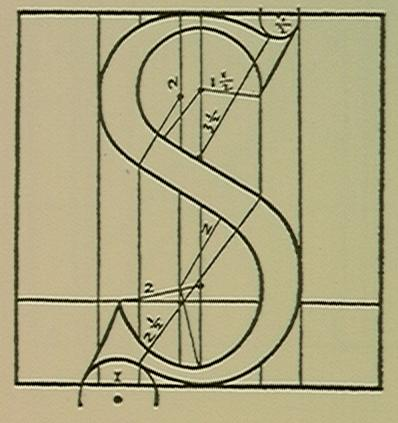
\includegraphics[width=.75\textwidth,height=.80\textwidth,keepaspectratio]{pictures/torniS}
\caption{토르니엘로의 S자 도해}\label{fig:orginal}}
\end{figure}

\begin{enumerate}
\item  중심이 $(4.5, 5.5)$이고 반지름이 $3.5$인 원호를 그린다. 이때
  $P_1$은 원호상의 점 $(4.5, 9)$이다. \label{p:first}


\item 이때 \ref{p:first}에서 그린 원호가 직선 $x=6$와 만나는 점을
  $P_2$라 하자. 그러면 $P_2$는 $(6, 5.5+\sqrt{(3.5)^2 - (1.5)^2})= (6, 5.5+\sqrt{10})$이다.

\item 중심이 $(6.5, 9)$이고 반지름이 $0.5$인 원호를 그릴 차례다. 원호상의
   점 $(6.5, 8.5)$를 $P_3$이라 하고 $P_3$에서 $(7, 9)$까지 원호를 그린다. 

\item 점 $(6, 7)$를 $P_4$이라 하고, $P_4$에서 방금 그린 원호에 접하는
  직선을 긋는다.\label{p:fourth}

\item \ref{p:fourth}에서 원호와 직선의 접점을 $P_5$라 하면  $P_5$는
 $\left (6\frac{16}{17}, 8\frac{13}{17}\right )$이다. (원의 성질과
 닮음비, 삼각비를 이용하여 방정식을 푼다.)


\item 중심이 $(4, 7)$이고 반지름이 $2$인 원호를 그린다. 이때 $P_6$과
  $P_7$은 각각 $(4, 9)$, $(3, 7-\sqrt3)$이다. 이 두 점 사이 만큼
  원호를 그린다.

\item $(5, 4)$를 $P_8$이라 하고 $P_7$에서 $P_8$까지 직선을 긋는다.


\item 중심 $(4.5, 7\frac{1}{8})$에서 $P_4$를 지나는 원호를 $P_9 = (3.5,
  6)$까지 긋는다. 

\item $(6, 4.5)$를 $P_{10}$이라 하고 $P_9$에서 $P_{10}$까지 직선을
  긋는다.

\item $P_{10}$을 지나고 중심이 $(4.5, 2.5)$이고 반지름이 $2.5$인
  반원을 그린다. $P_{11}$은 $(3, 0.5)$이다.

\item $P_{11}$과 $P_{12}$를 잇는  다른 작은 원호를
 그린다. 이 원호의 중심은 $(2.5, y)$이고 반지름은
  $1$인데, $P_{12}$의 $x_{12}$ 좌표는 $1\frac78$이다. 따라서
 $y=(1-\sqrt3)/2 \approx -0.37$이고 $y_{12}=(\sqrt{39}+4-4\sqrt{3}) / 8
 \approx 0.41$이다. (원의 방정식을 풀어야 한다.) 

\item $P_8$에서 (아직 정의되지 않은) $P_{13}$을 잇는 반지름이 $2$인
  원호를 그린다. 이 원호의 중심의 $x$ 좌표는 $4$이고 $x_{13}=
  4.5$이다. 원의 방정식을 풀면 중심은 $(4, 4-\sqrt3) \approx (4,
  2.27)$이고 $y_{13}=4-\sqrt{3}-\sqrt{3.75} \approx 0.33$이다. 

\item $P_{13}$에서 (아직 정의되지 않은) $P_{14}$를 잇는 반지름이 $2$인
  원호를 그린다. 이 원호의 중심의 $y$ 좌표는 $4.5$이고 $y_{14}=
  2$이다. 원의 방정식을 풀면 중심은 $(4.5, 6-\sqrt3-\sqrt{3.75}) \approx (4.5,
  2.33)$이고 $x_{14}=4.5-\sqrt{4-(4-\sqrt{3}-\sqrt{3.75})^2} \approx
  2.53$이다. 

\item 마지막으로 $P_{14}$와 $P_{12}$를 잇는다. 
\end{enumerate}

\bigskip
(인용 끝)


\section{그려보기}

\begin{itemize}

\item 그림~\ref{fig:illustrator}\은 \textsf{Adobe Illustrator}에서
  크누스 교수가 소개한 방법으로 그렸는데, 정확한 작도를 위해 약간의 원의 방정식을 풀어야 했습니다. 

\item 토르니엘로가 그린 다른  문자를 볼 수 있는 곳\\
	\url{http://rubens.anu.edu.au/htdocs/bytype/typefaces/torniello}

\end{itemize}

\begin{figure}
\centering{
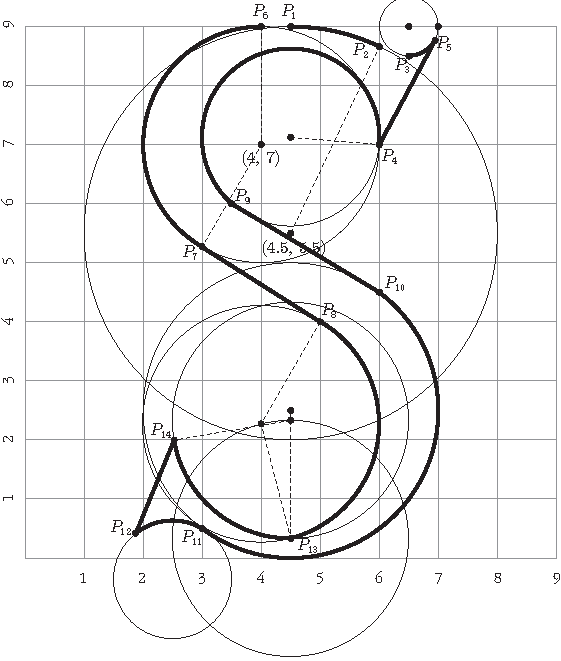
\includegraphics[width=.95\textwidth]{pictures/torniello}
\caption{크누스가 소개한 작도 방법으로 그려본 토르니엘로의 S자}
\label{fig:illustrator}}
\end{figure}

\begin{figure}
\centering{
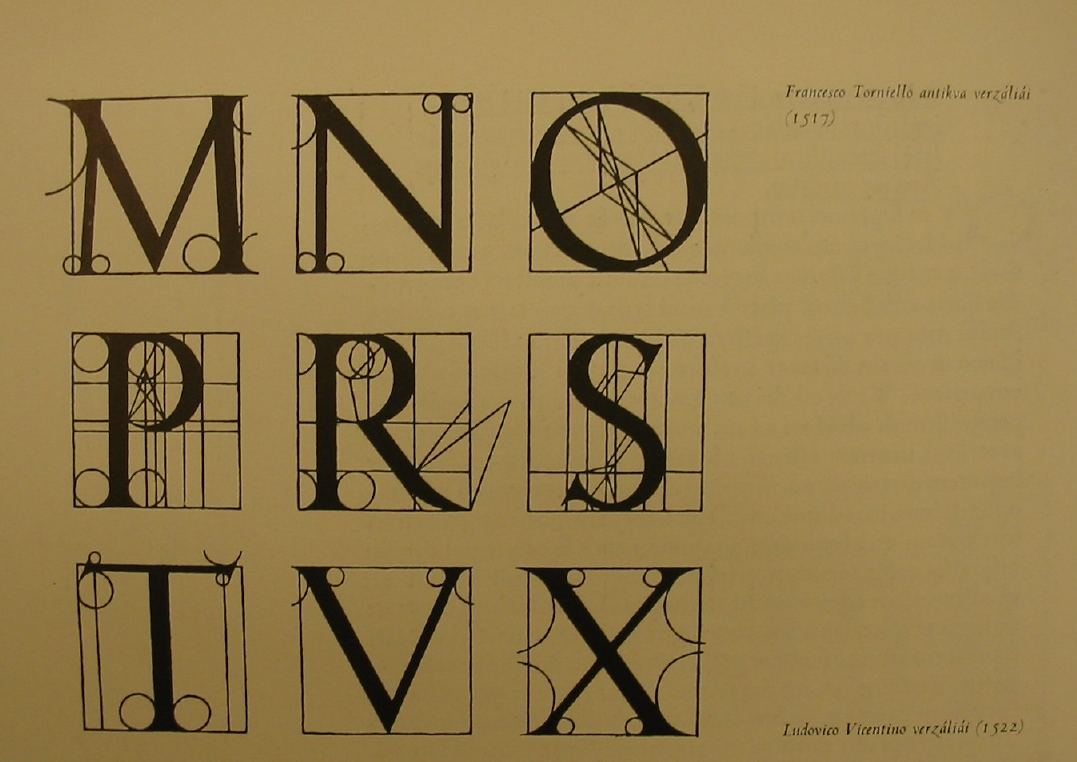
\includegraphics[angle=90, width=.95\textwidth]{pictures/otherletters}
\caption{토르니엘로의 다른 문자}
\label{fig:otherletter}}
\end{figure}
